
% ════════════════════════════════════════════
% 模型准备（5.1.2.模型准备.tex，三级子块）
% ════════════════════════════════════════════
\subsubsection{数据清洗与参数标定}

\textbf{1.数据预处理}

附件一给出了某一天不同时刻的电价、小区负载和光伏发电预测功率，时间分辨率均为 10 分钟，其中末行时间记作 $0{:}00{+}1$，表示当天 24:00。原始数据以时间字符串索引，无法直接用于逐时段递推计算，需先对齐时间并作数值化处理。将一天划分为 144 个等长时间间隔，第 $k$ 个间隔（$k=0,1,\dots,143$）对应时段 $[k\Delta t,(k+1)\Delta t]$，其中 $\Delta t=1/6$ 小时；设该间隔的负载功率为 $L_k$、光伏功率为 $S_k$、电价为 $p_k$，数据点 $(k+1)\Delta t$ 处记录的功率即为该间隔内的平均功率，其能量为该功率与 $\Delta t$ 之积。将时间边界 $0{:}00{+}1$ 映射为 24:00，并对三列数据统一执行数值化与缺失检查，预处理前后对比如图\ref{fig:preprocess1}所示。

\begin{figure}[H]
    \centering
    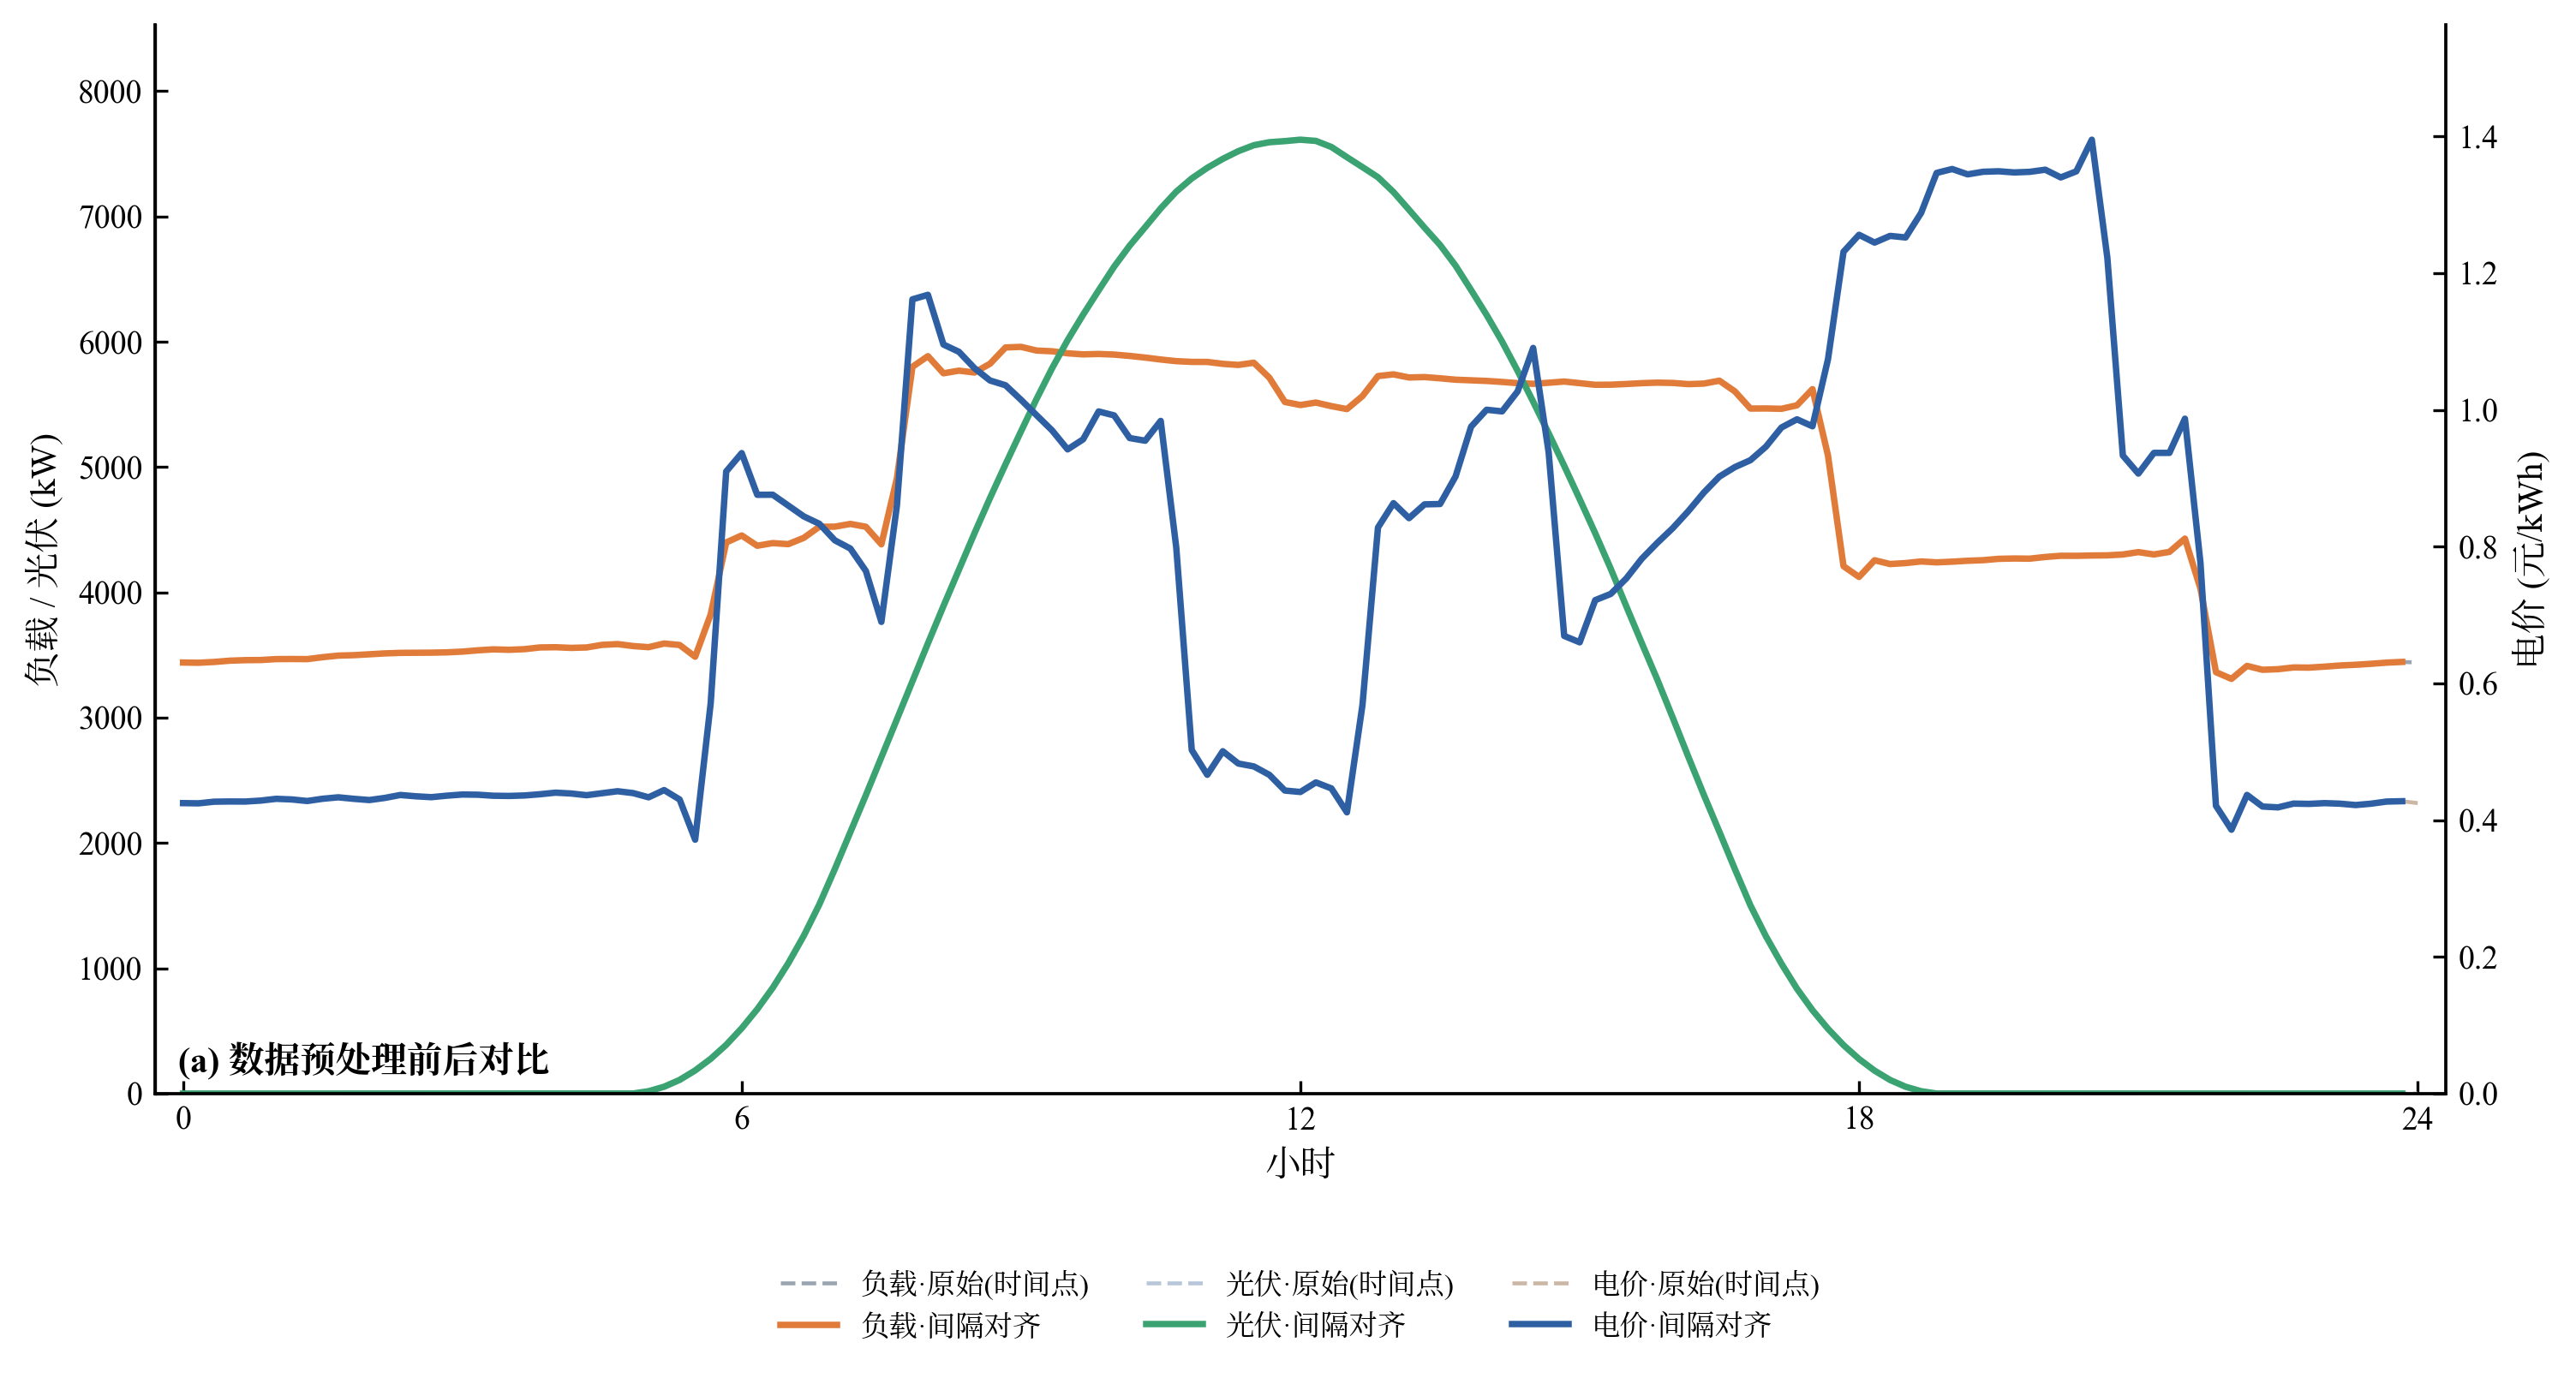
\includegraphics[width=0.46\textwidth]{求解/问题一/图片/图1-1_预处理前后对比.png}
    \caption{问题一数据预处理前后对比}
    \label{fig:preprocess1}
\end{figure}

预处理后电价、负载与光伏三条曲线均对齐到 144 个 10 分钟间隔上，数据无缺失、无异常，光伏功率在日出后至日落前呈现典型的单峰形态，为后续优化提供了可靠输入。

\textbf{2.算法选择}

微网购电调度是一个带线性约束的凸优化问题。枚举搜索理论上能找到最优解，但决策变量规模达数百个，计算量爆炸；贪心算法难以同时协调储能容量约束与日循环约束；线性规划能把所有线性约束与目标函数直接纳入模型，由单纯形法或内点法求得全局最优解\cite{si2011}，求解速度极快。据此，本问选择线性规划求解。
